% This is "sig-alternate.tex" V1.9 April 2009
% This file should be compiled with V2.4 of "sig-alternate.cls" April 2009
%
% This example file demonstrates the use of the 'sig-alternate.cls'
% V2.4 LaTeX2e document class file. It is for those submitting
% articles to ACM Conference Proceedings WHO DO NOT WISH TO
% STRICTLY ADHERE TO THE SIGS (PUBS-BOARD-ENDORSED) STYLE.
% The 'sig-alternate.cls' file will produce a similar-looking,
% albeit, 'tighter' paper resulting in, invariably, fewer pages.
%
% ----------------------------------------------------------------------------------------------------------------



% This .tex file (and associated .cls V2.4) produces:
%       1) The Permission Statement
%       2) The Conference (location) Info information
%       3) The Copyright Line with ACM data
%       4) NO page numbers
%
% as against the acm_proc_article-sp.cls file which
% DOES NOT produce 1) thru' 3) above.
%
% Using 'sig-alternate.cls' you have control, however, from within
% the source .tex file, over both the CopyrightYear
% (defaulted to 200X) and the ACM Copyright Data
% (defaulted to X-XXXXX-XX-X/XX/XX).
% e.g.
% \CopyrightYear{2007} will cause 2007 to appear in the copyright line.
% \crdata{0-12345-67-8/90/12} will cause 0-12345-67-8/90/12 to appear in the copyright line.
%
% ---------------------------------------------------------------------------------------------------------------
% This .tex source is an example which *does* use
% the .bib file (from which the .bbl file % is produced).
% REMEMBER HOWEVER: After having produced the .bbl file,
% and prior to final submission, you *NEED* to 'insert'
% your .bbl file into your source .tex file so as to provide
% ONE 'self-contained' source file.
%
% ================= IF YOU HAVE QUESTIONS =======================
% Questions regarding the SIGS styles, SIGS policies and
% procedures, Conferences etc. should be sent to
% Adrienne Griscti (griscti@acm.org)
%
% Technical questions _only_ to
% Gerald Murray (murray@hq.acm.org)
% ===============================================================
%
% For tracking purposes - this is V1.9 - April 2009

\documentclass{sig-alternate}
\usepackage{blkarray}

\usepackage{array}
\newcolumntype{L}[1]{>{\raggedright\let\newline\\\arraybackslash\hspace{0pt}}m{#1}}


\begin{document}
%
% --- Author Metadata here ---

\conferenceinfo{MM'12}{ October 29-November 2, 2012, Nara, Japan.}
%\CopyrightYear{2007} % Allows default copyright year (20XX) to be over-ridden - IF NEED BE.
%\crdata{0-12345-67-8/90/01}  % Allows default copyright data (0-89791-88-6/97/05) to be over-ridden - IF NEED BE.
% --- End of Author Metadata ---



\title{AMoViMash: Online Mobile Video Mashup}


\numberofauthors{8} %  in this sample file, there are a *total*
% of EIGHT authors. SIX appear on the 'first-page' (for formatting
% reasons) and the remaining two appear in the \additionalauthors section.
%
\author{
\alignauthor Mukesh Saini\\
       \affaddr{Dept. of Computer Science}\\
       \affaddr{National University of Singapore}\\
       \email{mksaini@comp.nus.edu.sg}
% 2nd. author
\alignauthor Raghudeep Gadde\\
       \affaddr{Dept. of ECE}\\
       \affaddr{National University of Singapore}\\
       \email{elerdg@nus.edu.sg}
\and  
% 3rd. author
\alignauthor Shuicheng Yan\\
       \affaddr{Dept. of ECE}\\
       \affaddr{National University of Singapore}\\
       \email{eleyans@nus.edu.sg}
% 4th. author
\alignauthor Wei Tsang Ooi\\
       \affaddr{Dept. of Computer Science}\\
       \affaddr{National University of Singapore}\\
       \email{ooiwt@comp.nus.edu.sg}
}
% There's nothing stopping you putting the seventh, eighth, etc.
% author on the opening page (as the 'third row') but we ask,
% for aesthetic reasons that you place these 'additional authors'
% in the \additional authors block, viz.

% Just remember to make sure that the TOTAL number of authors
% is the number that will appear on the first page PLUS the
% number that will appear in the \additionalauthors section.

\maketitle
\begin{abstract}
With the proliferation of mobile video cameras, it is becoming easier
for users to capture videos of live performances and socially
share them with friends and public. As an attendee of such live
performances typically has limited mobility, each video camera is
able to capture only from a range of restricted viewing angles and
distance, producing a rather monotonous video clip. At such performances,
however, multiple video clips can be captured by different
users, likely from different angles and distances. These videos
can be combined to produce a more interesting and representative
mashup of the live performances for broadcasting and sharing. The
earlier works select video shots merely based on the quality of currently
available videos. In real video editing process, however, recent
selection history plays an important role in choosing future
shots. In this work, we present MoViMash, a framework for automatic
online video mashup that makes smooth shot transitions to
cover the performance from diverse perspectives. Shot transition
and shot length distributions are learned from professionally edited
videos. Further, we introduce view quality assessment in the framework
to filter out shaky, occluded, and tilted videos. To the best
of our knowledge, this is the first attempt to incorporate historybased
diversity measurement, state-based video editing rules, and
view quality in automated video mashup generations. Experimental
results have been provided to demonstrate the effectiveness of
MoViMash framework.\\
\textbf{Categories and Subject Descriptors:} I.2.10 [Vision and Scene
Understanding]: Video Analysis\\
\textbf{General Terms:} Algorithms, Design.\\
\textbf{Keywords:} Mobile Video, Virtual Director, Video Mashup.
\end{abstract}



% A category with the (minimum) three required fields
%\category{H.4}{Information Systems Applications}{Miscellaneous}
%A category including the fourth, optional field follows...
%\category{D.2.8}{Software Engineering}{Metrics}[complexity measures, performance measures]

%\terms{Theory}

%\keywords{ACM proceedings, \LaTeX, text tagging}

\section{Introduction}
Worldwide shipment of camera phones were estimated to reach
1.14 billion in the year 2011 alone \cite{1}. Furthermore, a survey of over 2,500 respondents by Photobucket reveals that 45\% of the respondents use mobile devices to shoot video at least once weekly during the summer of 2011, validating the significant increase in the amount of mobile video uploaded to Photobucket's video sharing website (14$\times$ in Summer 2011 compared to December 2010) \cite{2} .

Proliferation of such mobile devices with video capture capability has enabled users to capture video of their life events such as concerts, parades, outdoor performances, etc, and socially share
them with friends and public as it happens. Videos recorded by a single user at such events are shot from a limited range of angles and distances from the performance stage, as an attendee typically has limited mobility (e.g., constraint by seating arrangement).

The recorded video can be monotonous and uninteresting. Furthermore, videos recorded are typically short (in the order of minutes or tens of minutes), due to tired arms or power constraint of mobile devices. There are, however, likely to have more than one users
recording the same performance from different angles at the same
time, especially at a well-attended performance.
These recorded and shared video clips of the same performance
can be cut and joined together to produce a new mashup video, similar to how a TV director of a live TV show would switch between different cameras to produce the show. Generation of a video mashup can be cast as a video selection problem: given a set of video clips capturing the same performance event, automatically select one of the video clips at any one time instance to be included in the output mashup video.

In this paper, we introduce MoViMash, our approach to solve
the above video selection problem. MoViMash aims to produce
mashup video from a set of mobile devices that is interesting and
pleasing to watch, and uses a combinations of content-analysis,
state-based transitions, history-based diversity, and learning from
human editors to achieve this goal.

We now provide an overview of how MoViMash works in the
usual setting of live performances, shown in Figure \ref{fig:figrue1}. There is
generally a staging area and an audience area where the audiences either sit or stand to watch the performance, and record the performance with a mobile device. This setting poses a few challenges to video mashup.

\begin{figure}[h]
    \centering
    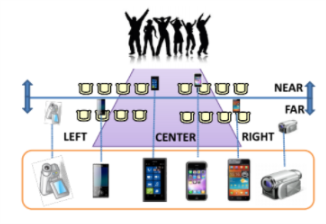
\includegraphics[width=0.5\textwidth]{img1.png}
    \caption{A general performance scenario}
    \label{fig:figrue1}
\end{figure}

Since the videos are recorded with a hand-held mobile device,
from the audience area, and likely by non-professional, there is no
guarantee on the view quality. The videos can be shaky or tilted.
Furthermore, it is common to include the back of the head of other
audiences in the view. As other audiences move, the view can be
temporarily occluded. When MoViMash needs to decide which
video to select, it first filters out the videos with bad views currently from further consideration for selection. To achieve this, MoViMash analyzes the video to determine the current shakiness, the tilt angle, and the level of occlusion in the video. Note that shakiness and tilt angle can be obtained from easily sensory data of mobile device when available.



The shooting angle of the remaining videos are then classified as
either center, left, and right; and distance from the stage as near and
far as shown in Figure \ref{fig:figrue1}. This classification is done every time we perform video selection because mobile users may change their position over time. MoViMash now decides which shooting angle and distance should be used; and for how long the selected class should persist. To this end, MoViMash tries to imitate a professional video editor, by using a finite state machine, whose transition probabili ties are learned from analyzing professionally edited videos of the same type of event. The rationale behind the inclusion of learning is that, we have observed that there are no generic editing rules that can be precisely defined to work with all types of events. The video editors make fine decisions such as shot lengths and transitions based on their experience which is hard to enumerate.

The videos from the selected class are further ranked based on
the video quality and diversity values to make the final selection. To consider video quality, MoViMash favors video with low blurriness, low blockiness (good compression), good contrast, and good illumination in each video. To consider diversity, MoViMash stores a history of recent video selections and favors videos with dissimlar views with recent selections.

We have developed MoViMash's algorithm such that it is online
and only depends on history information. As such, even though
it is not our main goal in this paper, MoViMash can be applied to
mashup of live video feeds from mobile devices.

We now briefly compare MoViMash to existing work to high light the contribution of this paper. There has been few works on video selection in a lecture broadcast and video streaming \cite{21} \cite{6}
and video conferencing \cite{3}. In these works the camera is mainly
selected based on speaker detection. Live performances are not
speaker centric. In fact, the speech signals are generally noise from
the crowd. In one recent work, Shrestha et al. \cite{15} propose a method to create a video mashup from a given set of concert recordings. In that work, the authors select the shots based on mainly video quality, mostly ignoring view quality. Also, the diversity is only calculated based on the comparison of the last image of the current shot and first image of the next shot. It does not consider the history of video selection and the time for which a particular camera is selected. Further, video editing rules, which are subtle in the case of live performances, are not considered. 

\textbf{Contributions.} We now summarize our contributions in this paper as follows:

\begin{itemize}
\item We propose a state-based approach for shot selection that in-
corporates the selection history in the decision process. Earlier methods select shots based on only currently available videos.
\item  We include view quality in the framework to filter out the
bad views that are occluded, tilted, or shaky. Earlier methods
only considered video quality.
\item  We build a comprehensive model to calculate diversity that
considers both previously selected videos and shot lengths.
\item  We propose a learning-based approach where the shot tran-
sition probabilities and shot lengths are learned from profes-
sionally edited videos.
\end{itemize}

\textbf{Organization.} The rest of the paper is organized as follows.
We provide a review of earlier work in Section 2. In Section 3 we
describe proposed mashup framework. We evaluate our system in
Section 4. The conclusions are provided in Section 5.

\section{PREVIOUS WORK}
There has been only few works on online camera selection. In most of these works, videos are mainly selected to show the speakers. In the work by Machnicki and Rowe \cite{9}, an online lecture webcast system is presented in which the cameras that are focusing on speaker and the presentation (the screen) are selected iteratively until anybody from audience asks question. When audience ask question, the camera that is focusing the person asking question is selected. The automatic selection of cameras in a lecture webcast is extended by Zhang et al. \cite{21} to include audio based localization and speaker tracking. Similar approach is taken by Cutler et al. \cite{6} in a meeting scenario where camera that shows the current speaker is selected. Ranjan et al. \cite{12} use face tracking and audio analysis to show the close-up of the person talking. Since performers play more important role than speakers in live concerts, a speaker based selection is not appropriate. Further, the faces are generally far from the camera which cannot be detected. Therefore, face detection is not a reliable basis to select videos.




\begin{table*}
\centering
\caption{A Comparison of Previous Work}
\begin{tabular}{c|c|c|c|c|c|c} \hline
Work&Online&Diversity&Learning&Video Quality&View Quality&Scenario\\ \hline
\texttt Machnicki et al. \cite{9}&Yes&No&No&No&No&Lecture webcast  \\ \hline 
\texttt Cutler et al. \cite{6}&No&No&No&No&No&Meeting  \\ \hline 
\texttt Al-Hames et al. \cite{3}&Yes&No&No&No&No&Meeting  \\ \hline 
\texttt Yu et al. \cite{20}&Yes&No&No&No&No&Lecture webcast  \\ \hline 
\texttt Zhang et al. \cite{21}&Yes&No&No&No&No&Lecture webcast  \\ \hline 
\texttt Wang et al. \cite{16}&Yes&No&No&Yes&No&Sports Broadcast  \\ \hline 
\texttt Engstrom et al. \cite{8}&Yes&No&No&No&No&Sports Broadcast  \\ \hline 
\texttt Lima et al. \cite{7}&No&No&No&No&No&Storyline  \\ \hline 
\texttt Ranjan et al. \cite{12}&Yes&No&No&No&No&Meeting  \\ \hline 
\texttt Shrestha et al. \cite{15}&No&No&No&No&No&Live Performances  \\ \hline 
\texttt \textbf{Proposed}&Yes&Yes&yes&Yes&Yes&Live Performances\\ \hline
\end{tabular}
\end{table*}




Al-Hames et al. \cite{3} extends the camera selection work to include the motion features. We do not use motion features in our framework because both performers and audience generate continuous motion. Also, the movement of the mobile camera can inject erroneous motion in the video, which is aesthetically appealing. Yu et al. \cite{20} propose to customize the camera selection and shot lengths based on user preferences. At every lecture webcast receiving site, the user can give score to the videos and specify rules for shot lengths. While such an interactive selection of cameras is useful for educational scenarios, people may find it annoying and stressful for performances, particularly when the number of videos is large.

A camera selection method for sports video broadcast is proposed by Wang et al. \cite{16}. The authors assume one main camera and other sub cameras. The empirical main camera duration is found to be from 4 to 24 seconds, and sub camera duration is found to be 1.5 to 8 seconds. They select a sub camera based on the clarity of the view, determined using motion features. In our work, along with shakiness of the videos, we also calculate view quality in terms of occlusion and rotation; and video quality in terms of contrast, blur, illumination, and blockiness. We also include explicit measurement of diversity in the framework. Engstrom et al. \cite{8} discuss automatic camera selection for broadcast in a sports event capture scenario. The work mainly promotes collaborative
video production, i.e., video recorded by production team as well
as the consumers.

In other media production applications, the shots are selected to
convey the story to the audience. For instance, de Lima et al. \cite{7} propose a method to automatically select shots from multiple cameras for storytelling, according to the rules provided by the director.
These methods are not useful for us as live performances generally
do not have any story.

Recently, there has been works on creating video mashups from
given set of videos. In one of the most recent works \cite{15}, Shrestha et al. select the cameras based on video quality. Although the authors refer to term 'diversity' in the paper, it is merely a comparison of current frame and the next frame of the corresponding camera. The authors completely ignore the selection history and the time for which each view is selected. The authors also ignore editing rules corresponding to different views, which we incorporate through learning based classification and selection. Furthermore, unlike the method proposed in this paper, the authors rely on the future video for current shot selection. While this approach is fine for combining stored videos, it is not suitable for live applications
such as broadcasting and live sharing.


\begin{figure}[h]
    \centering
    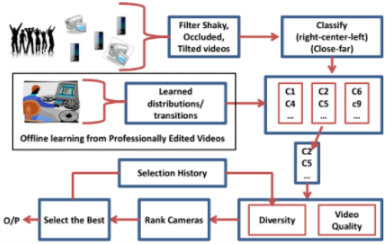
\includegraphics[width=0.5\textwidth]{img2.png}
    \caption{The virtual director framework}
    \label{fig:figure2}
\end{figure}


We have provided a comparison of the related work in Table 1. The works have been compared with respect to the following aspects: (1) can the method be applied online (a method that uses future information cannot be applied online)? (2) is selection historybased diversity considered? (3) is learning incorporated? (4) is video quality (clarity, contrast etc.) considered? (5) is view quality (view occlusion, tilted view etc.) considered? and (6) what is the underlying application scenario? It can be easily seen that the proposed method is the first attempt to consider history based diversity through learning for online video selection for live performances.





\section{MOVIMASH FRAMEWORK}
In this section, we first enumerate the design principles that we
have followed in the development of MoViMash and then describe the framework. After an overview of MoViMash, we focus on individual components.

\subsection{Design Principles}
The end goal of the MoViMash is to produce a mashup that users like. To achieve this goal, we have followed a set of design principles as follows:

\begin{itemize}
\item \textbf{Video Quality:} In our discussion, video quality includes
sharpness, contrast, illumination, and blockiness (due to video compression). A good image quality gives pleasing experience to the viewers \cite{10}. Therefore, in our framework we give priority to good quality videos.
\item \textbf{View Quality:} A video that is captured by a tilted camera (rotated around horizontal axis) may have very good video quality, yet, users generally do not like tilted views. Similarly, a view in which a person or object is occluding stage area (blocking performance view) may be annoying to the user. Therefore view quality is also important. We measure view quality in terms of occlusion, tilt, and shakiness.
\item \textbf{Diversity:} While static cameras always record videos fromsame perspective, mobile users generally shoot videos from a number of views and diverse perspectives. We take this opportunity to include more diversified views in the mashup. Both temporal and spatial aspects of diversity are considered in the proposed framework.
\item \textbf{Learning:} When professionals edit the videos, they make
many decisions based on their experience. Such decisions include shooting angle, distance from the stage, and shot length. It is, however, difficult to precisely state this experience in terms of hard-coded rules. Therefore, in this work, we learn the shot transitions and lengths from professionally edited videos.
\end{itemize}

The above mentioned design principles are met in our framework through various quality metrics and video selection/filtering phases, as described in the following section.

\subsection{Framework}
At every time instant, we have a number of videos to choose from. Once we have chosen the video, we also need to decide when to switch to another video. Hence, there are two main questions involved here that need to be answered for combining videos: (1) which video to select? (2) when to switch to another video? We use a three-phase method to select the video while the length is determined based on learned editing rules and overall quality score of the selected video.

Figure 2 shows the block diagram of overall framework. The proposed framework consists of one offline learning phase and three online selection phases namely filtering, classification, and selection. At any given time, the following steps are taken to select the most suitable video at current instant:

\begin{enumerate}
  \item \textbf{Filtering:} In the filtering step, we determine videos that are unusable by comparing occlusion, shakiness, and tilt scores
against empirically determined thresholds. The remaining videos are passed to the classification stage.
  \item \textbf{Classification:} The selected cameras are classified as one of right, center, and left according to the capturing angle. Further, according to the viewing distance from the stage, they are classified as near or far.

\item \textbf{ Class Prediction:} According to the class of currently selected video, and class transition probabilities learned from professionally edited videos, a most suitable class is predicted and videos from that class are selected for further consideration.

\item \textbf{Video Selection:} The classified cameras are further ranked with respect to a combined score of video quality, diversity,
and shakiness. The video with highest score is selected.

\item \textbf{Shot Length:} The length of the video is selected based on learned distributions and video quality. A higher quality video is generally selected for longer time.
\end{enumerate}

While filtering and selection phase ensure view and video quality, the classification and diversity ensure that we select videos recorded with different angles and viewing distances to provide a complete and interesting coverage of the performance. We now describe each component of the framework in detail.

\subsection{View Quality}
The view quality is measured in terms of three characteristics:
occlusion, shakiness, and camera tilt. The details of measurement
of each of these quantities is given below.

\subsubsection{Occlusion}
For both a stand mounted camera and a mobile camera, there is always a chance of view occlusion. At crowded places, people sometime do not notice the cameras recording the video and occlude the performance view. Even if people notice the cameras, they stand in front of or walk across the cameras, because the main purpose of the performances is to entertain the audience who are present at the venue rather than video recording. Therefore, we detect the videos which are recorded by occluded cameras and filter them out.

Occlusion detection methods are popular in the field of object tracking [13, 19]. There methods employ various appearance models to seamlessly track multiple objects. In this case, the occlusion occurs when an object is hidden behind another. In live performances, this could be intentionally done by the performers, i.e., one performer coming in front of other. We are more interested in detecting the audience blocking the view. Therefore, those works are not applicable here.

We have developed an edge density based method to detect videos with occluded views. The method is based on the assumption that the objects that occlude the performance area will result in lower edge density than the performance area. Therefore, the non-occluded area of the image, which is far from the camera, will result in more dense edge points than the occluded area. To differentiate between homogeneous regions of the stage area, which could also have less edge density, and occluded area; we perform connected components on the edge image. Following are the steps of the occlusion detection in a given image I:

\begin{itemize}
\item Edge Detection: In the first step, we calculate the presence of
an edge at each pixel location. Let $I^e$ be the resulting binary
edge image :

\begin{equation}
I^e(x,y) =
\begin{cases}
  1  & \text{if edge is detected at pixel I(x, y)}\\
  0  & \text{otherwise}
\end{cases}
\end{equation}
\end{itemize}  





\begin{figure}[h]
    \centering
    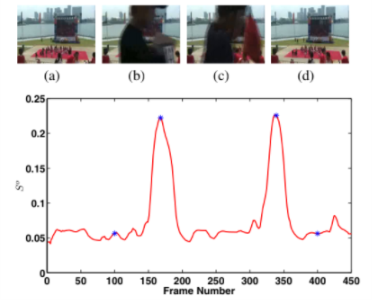
\includegraphics[width=0.5\textwidth]{img3.png}
    \caption{Occlusion detection. Figures (a)-(d) show the frames
100, 168, 339, and 400 of the test video respectively. Figure (e)
shows the corresponding occlusion score}
    \label{fig:figure3}
\end{figure}

  
\begin{itemize}  
\item Edge Density: We convolve the edge image with a square
matrix W with all of its elements unity:

\begin{equation}
    I^D = I^e \odot W
\end{equation}
The output of the operation gives the density of edges around
each pixel.
\end{itemize}

\begin{itemize}
\item Labeling the Patches: The image is now divided into patches
of block size $b \times b$.
Each patch is labeled as 1 if the sum of
edge densities is less that a threshold, else it is labeled as 0.
\end{itemize}


\begin{equation} I^p(x',y') =  
\begin{cases}
      1  &  \text{if the sum of edge densities in the}\\
         &  \text{patch (x',y') is greater than threshold}\\
      0  &  \text{otherwise}
\end{cases}  
\end{equation}

The 1's in the patch image shows potentially occluded regions.

\begin{itemize}
\item Connected Components: There can be homogeneous regions
in the non-occluded area as well. These regions, however, are
generally small. Therefore, connected components operation
is performed to find the size of largest group of connected
patches with label 1, which corresponds to occluded region.

\item Occlusion Score: To calculate the final occlusion score $S^o$ , we first calculate the fractional occluded region f in the connected components output image, i.e.,
\end{itemize}

\begin{equation}
    f =  \frac {No \ of \ 1 \ patches}{Total \ number \ of \ patches} 
\end{equation}

We also observed that generally the dynamic range of f is very
small. Therefore, we expand its range with an exponential function
to calculate the final score $S^o$:

\begin{equation}
    S^o = {1 {-} {e}^{{-}f}}
\end{equation}


\begin{figure}[h]
    \centering
    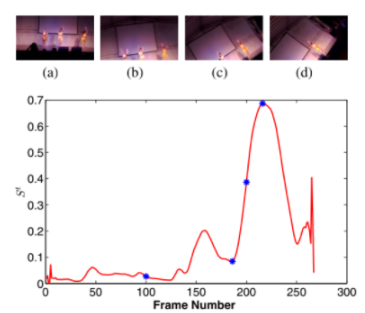
\includegraphics[width=0.5\textwidth]{img4.png}
    \caption{Tilt results. Figures (a)-(d) show the frames 100, 186,
200, and 286 of the test video respectively. Figure (e) shows the
corresponding tilt score}
    \label{fig:figure4}
\end{figure}


The resulting occlusion scores for an example video sequence
are shown in the Figure 3. The sequence shows a person walking
across a camera, which is recording an outdoor performance. We
can see that as the person enters the camera view, the occlusion
score starts increasing. We obtained similar results for night videos
also, which are not shown due to space limitation. We found that
for a patch size of 20*15 pixels, videos with occlusion score more
than 0.2 are very bad, so these are filtered in the framework.

\subsubsection{Tilt}
In this work, we define tilt as the rotation of the camera around
horizontal axis. User's generally do not like the videos recorded
by tilted cameras. Therefore, we detect the tilted camera views
and filter them. Here we use the heuristic that for a horizontally
placed camera, most of the lines in the view are horizontal, while
an inclined view generally has non-horizontal lines. The following
steps are taken to calculation tilt:

\begin{itemize}
\item Line Detection: We use Hough transform to detect the straight
line in the image. Let $l'_i$ be the length of the $i^{th}$ line and $o'_i$ the angle with respect to the horizontal line.
\item Angle Restriction: We assume that the maximum tilt a camera can have is less than $\pm \pi/4 $ and any line with the inclination above this angle is noise and not considered in calculation. Let the resulting orientation of $l'_i$ line be $o'_i$.
\item The final tilt score $S^t$ is calculated as absolute of the mean
weighted orientation and normalized by $\pi/4$:
\end{itemize}

\begin{equation}
    S^t = \frac{abs \Big(\frac{1}{N^l} \sum_{i=1}^{N^l} o^i * l^i\Big)}{\pi/4}
\end{equation}

where $N^l$ is the total number of lines in the image.\\

An example of tilt calculation is shown in Figure \ref{fig:figure4}; the upper
row shows frames from the video and the figure in lower row shows
occlusion scores. The video clip is recorded by a mobile phone
camera. In between, the mobile user gets engaged in some other
activity, and the mobile phone gets tilted. We can observe in the
frames itself the straight lines getting tilted. It gets reflected in the
tilt score as shown in Figure \ref{fig:figure4} for frames 200 and 216. The videos
with a tilt score of 0.4 are found unusable and they are filtered.

\subsubsection{Shakinesss}
Shakiness is calculated based on the method described in \cite{4}.
In this method, the pixel values are projected on horizontal and
vertical axes. The horizontal and vertical projections are matched
across the frames for calculating camera motion. A median filtered
is finally applied on the motion vectors to differentiate the shakiness from the smooth camera motion. The final value of shakiness
score, $S^8$, is calculated by summing the absolute difference of original motion vector and median filtered motion vector. The score is
normalized by calculating maximum difference empirically. For a
shakiness window of 100 frames, the normalization value is 300;
for any value above 300, $S^8$ is saturated to 1.

\subsection{Learning}
As mentioned earlier in Section 1, it is difficult to precisely enumerate all the rules which professional editors follow in selecting
a video and its corresponding shot length. In MoViMash, we propose to learn the behavior of professional editor statistically for use
in creating mashup. We use professionally edited videos for this
purpose. The rules are learned in terms of shooting angle, shooting distance, and shot length. Following are the steps taken in the process of learning:

\begin{itemize}
\item At first, we divide the video into a sequence of shots and
record shot length.
\item Each shot is classified as right (R), left (L), or center (C)
based on shooting angle (Figure 1).
\item Depending on the distance of the recording device from the
stage, the videos are further classified as near (N) or far (F) (Figure 1).
\item on both classifications, we define six states (also referred as classes in the paper) in which a video can be at any time instant, i.e., CN , CF, RN , RF, LN , and LF.
\item From the sequence of the shots, we calculate the state transition probabilities for the above described six states.
\item We now feed the transition probabilities (transition matrix)
along with shot lengths (emission matrix) to an hidden Markov
model (HMM). The HMM generates a sequence of shot states
and their corresponding lengths.
\end{itemize}


\begin{equation}  
\begin{blockarray}{ccccccc}
        & CN & CF & RN & RF & LN & LF\\
\begin{block}{c(cccccc)}
      CN & 0 & 0.4 & 0.2 & 0.1 & 0.2 & 0.1 \\
      CF & 0.6 & 0 & 0.1 & 0.1 & 0.1 & 0.1 \\
      RN & 0.5 & 0.1 & 0 & 0.1 & 0.2 & 0.1 \\
      RF & 0.2 & 0.2 & 0.4 & 0 & 0.1 & 0.1 \\
      LN & 0.4 & 0.2 & 0.2 & 0.1 & 0 & 0.1 \\
      LF & 0.2 & 0.2 & 0.1 & 0.1 & 0.4 & 0 \\
\end{block}
\end{blockarray} 
\end{equation}



\begin{equation}  
\begin{blockarray}{cccccccc}
        & 1 & 2 & 3 & 4 & 5 & 6 & 7\\
\begin{block}{c(ccccccc)}
      CN & 1/31 & 2/31 & 4/31 & 7/31 & 7/31 & 6/31 & 4/31 \\
      CF & 3/12 & 4/12 & 2/12 & 1/12 & 1/12 & 1/12 & 0    \\
      RN & 2/15 & 3/15 & 4/15 & 3/15 & 2/15 & 1/15 & 0    \\
      RF & 3/10 & 4/10 & 2/10 & 1/10 &   0  &   0  & 0    \\
      LN & 2/15 & 3/15 & 4/15 & 3/15 & 2/15 & 1/15 & 0    \\
      LF & 3/10 & 4/10 & 2/10 & 1/10 &   0  &   0  & 0    \\
\end{block}
\end{blockarray} 
\end{equation}

We use affine transformation to classify the video, giving an accuracy of $\approx 77\%$ on our dataset. However, since learning is one time job, we performed manual classification of shots during the
learning phase to get accurate statistics. Equation 7 shows the
learned transition matrix while Equation 8 emission matrix. We
have carefully selected five videos (live group dances with length of videos ranging from 210 to 300 seconds), which are professionally edited and aired on television. We downloaded these videos from YouTube.

These videos include concerts by professional bands and performance at the Academy Awards ceremony. We observed that in dance videos, the shot lengths are relatively smaller ( average around 2.3 seconds) compared to solo singing videos ( average around 3.5 seconds). This finding implies that the learning dataset should comply with the type of performance for mashup. We also observed that the average shot lengths for all five dance videos ranged between 2.2 seconds to 2.4 seconds, showing little variations, which shows that a particular type of events have similar pattern of transitions and shot lengths which can be learned and applied to create online mashup.


\subsection{Video Quality}
We can have different quality videos because of the limitation of
recording devices, varied camera positioning, lighting conditions, camera angle, and video recording skills of the person. To produce aesthetically beautiful video, it is important to consider the quality of the videos.We are considering the following aspects to obtain video quality score:

\begin{itemize}
\item \textbf{Blockiness:} The blocking effect mainly comes due to poor quality of data compression. To measure blockiness, we take current image as sample and calculate its compression quality using the method described in \cite{18}. The method generates
a score that takes a value between 1 and 10 (10 represents the
best quality, 1 the worst). We normalize the score between 0
and 1. Let Sb be the blockiness score.
\item \textbf{Blur:} The video can be blurred due to many reasons such as out-of-focus recording, camera movement etc. We are calculating blur based on the method described in \cite{5}. Let Sbr be the blur score which varies between 0 to 1 (0 represents
blurred and 1 sharp).





\item \textbf{Illumination:} There can be videos that are recorded in poor lighting conditions. The purpose of including this metric in quality measurement is to avoid selecting dark videos. The illumination score for the image $S^im$ (with width $N_w$ and height $N_h$) is calculated as average gray value, normalized by 255.

\begin{equation}
    S^{im} = \frac{1}{255}\frac{1}{N^w*N^h}\sum_{x=0}^{N^w}\sum_{y=0}^{N^h}I(x,y)
\end{equation}

\begin{figure}[h]
    \centering
    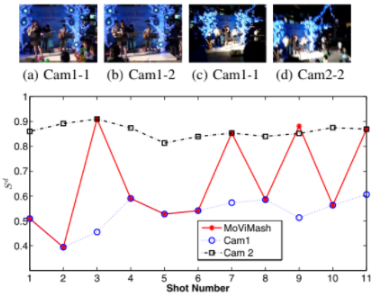
\includegraphics[width=0.5\textwidth]{img5.png}
    \caption{Diversity value for two candidate videos and final mashup}
    \label{fig:figure5}
\end{figure}


\item \textbf{Contrast:} It has also been found in the literature that an image with good contrast is appreciated by the viewers \cite{10}. Therefore, contrast is also chosen as one of the metrics. The contrast score $S^c$ is calculated as standard deviation of the pixel intensities.

\begin{equation}
    S^{im} = \frac{1}{255}\sqrt{\frac{1}{N^w*N^h}\sum_{x=0}^{N^w}\sum_{y=0}^{N^h}(I(x,y) - \bar{I})^2}
\end{equation}
Its value varies from 0 to 1 where 1 is the desired value cor-
responding to high contrast.

\item \textbf{Burned Pixels:} It has been identified that pixels that are
close to 255 or 0 are generally not informative \cite{15}. If $N^b$
is the number of such pixels, the quality score representing
burnt pixels is calculated as follows:

\begin{equation} S^{bp} = 
\begin{cases}
      1-N^b/(0.25*N^i)  &  \text{if} (0.25*N^i) < 1\\
       0                &  \text{otherwise}
\end{cases} 
\end{equation}

where $N^i$ is the total number of pixels in the image. In this
case, a value of 1 represents best quality, i.e., no burnt pixels;
while a value of 0 means at least 25\% pixels are burnt.

\end{itemize}

The individual quality scores are multiplied to calculate overall
video quality score $S^q$, i.e.,

\begin{equation}
    S^q = S^b \times S^{br} \times S^{im} \times S^c \times S^{bp}
\end{equation}

We have chosen to multiply the individual scores because we
want to give priority to the videos that are good in all aspects.

\subsection{Diversity}

The aspect of diversity is included in the framework by calculating the similarity of the views of the videos selected in the recent past. Let $\mathcal{H}$ be the history of the cameras that have been selected so far. The history is stored as set of chronologically order tuples, i.e.,

\begin{equation}
    \mathcal{H} = \{(I_{j}^{h} , \Delta _j )|1 \leq j \leq N^v\}
\end{equation}

where $N^v$ is the number videos selected in the recent past. Each
tuple has the following two entries:






\begin{itemize}
    \item $I^h$ - Snapshot from the selected cameras at the time of selection.
    \item $\Delta$ - The time for which the particular camera is selected. It is normalized between 0 to 1 by dividing each video duration by the total time over which history is stored.
\end{itemize}

Let $V S$ be the view similarity matrix:

\begin{equation}
    V S = \{v_{ij} |1 \leq i \leq n; 1 \leq j \leq N^v; \forall i = j, v_{ij} = 1\}
\end{equation}


where $n$ is number of cameras, and $v_{ij}$ is the view similarity
measure between current frame from the $i^{th}$ video and $j^{th}$ frame
of the history. The motivation of defining the view similarity $V S$ is
to select video with different views. The overall steps of diversity
calculation are as follows:


\begin{table}
	\caption{Details of the dataset}
	\begin{tabular}{L{1cm}|L{1cm}|L{1cm}|L{1cm}|L{1cm}|L{1cm}} \hline
		Performance&Type&Recordings&Duration(m)&Frame Rate&Resolution\\ \hline
		\texttt P1&Group Dance&12&4'&30&720*480 \\ \hline 
		\texttt P1&Group Dance&12&4'&30&720*480 \\ \hline 
		\texttt P1&Group Dance&12&4'&30&720*480  \\ \hline 
	\end{tabular}
\end{table}

\begin{enumerate}
    \item Determine the view similarity matrix $V S$ by comparing current frame with the frames stored in the history, i.e.,
    
    \begin{equation}
        v_{ij} = Diff(I^{c}_{i} , I^{h}_{j} )
    \end{equation}
    
    where $I^{c}_{i}$ is the current frame of  $i^{th}$ camera, $I^{h}_{j}$ is the  $j^{th}$ frame of the history, and $Diff$ can be any function to calculate view similarity. We are using \textbf{SSIM}\cite{17} for this purpose.
    
    \item For the given content, the user interest decreases with time
over which the user watches same or similar content. Hence,
the diversity score of the $i^{th}$ video, i.e., $S^d$ is calculated for each of the current videos as follows:

    \begin{equation}
        S^d = \sum_{j=1}^{N^v}v_{ij}*\Delta _j
    \end{equation}
    
    \item Store the viewing time of the previous video and the current
frame of the selected video in $\mathcal{H}$. If we choose a scheme
where each camera is selected only for fixed amount of time,
we may just store the current frame of the selected video.
    
\end{enumerate}

The diversity scores for two candidate videos (Cam 1, Cam 2)
and final mashup created using MoViMash for a performance (P3
in Table 2) are shown in the Figure 5. Although we are showing
diversity for only two videos for clarity, there were five candidate
videos in total. We can see that whenever a video gets selected,
its diversity generally reduces, e.g., diversity of Cam 1 after Shot 8
and diversity of Cam 2 after Shot 3. At Shot 4, Cam 1 gets selected
despite low diversity because its video quality is much better than
others (Figure 5.a-b) with a stable view. Sometimes the diversity
increases even when the video is currently selected (Shot 2, Cam 1)
due to change in camera view, or when one of previous selections
of the video moves out of history window. The diversity of Cam 2
decreases even though it is not selected. It is because during this
time, its view is similar to Cam 1, resulting in large (near 1) value
of $v_{12}$ (Equation 15). At Shot 9, a third (other than Cam 1 and Cam
2) video gets selected until Cam 1's diversity increases enough so
that it gets selected again. In summary, the metric $S^d$ is able to
capture and spatial and temporal diversity of videos.


\begin{figure*}[h]
    \centering
    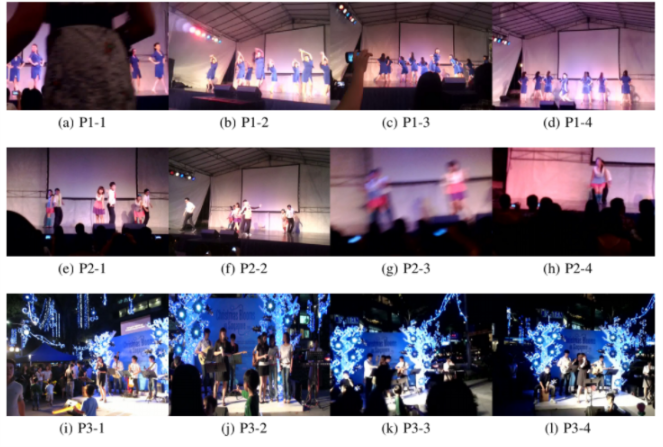
\includegraphics[width=01\textwidth]{img6.png}
    \caption{Selected frames from the recordings: (a-d) P1, (e-h) P2, (i-l) P3}
    \label{fig:figure6}
\end{figure*}


\subsection{Final Ranking}

For all the videos of the selected class, we have three metrics:
video quality score, diversity score, and shakiness score. We calculated weighted sum of these values to calculate final score $S^f$ :

\begin{equation}
    S^f = \alpha_1S^q + \alpha_2S^d + \alpha_3(1 - S^s)
\end{equation}

where $\alpha$1, $\alpha$2, and $\alpha$3 are weighting coefficients and $\alpha$1 + $\alpha$2 + $\alpha$3 = 1. In the experiments, we are using $\alpha$1 = $\alpha$2 = $\alpha$3 ,which gives equal weightage to the quality, diversity, and stability of the videos. Nevertheless, these coefficients should be determined based on the type of performance. For instance, in a hip-hop video mashup we can give less weightage to shakiness for better diversity and quality. A shaky video, however, can be annoying if the performance has smooth movements such as a tango performance.
We therefore need to keep $\alpha$3 higher in this case. Furthermore, if
the videos are generally bad in the quality, we can give set high
value for $\alpha$1. The shot from the video with the highest score is
selected at the current time instant.

\subsection{Length Selection}

To determine the switching instant, we are using a method which
combines the learning based prediction to obey the editing rules and
the superiority (in terms of overall quality) of the currently selected
video. As discussed in the learning section (Section 3.4), every
class of the videos follows a length distribution. For example the
center videos are generally selected for longer duration while the
left and right videos for relatively smaller duration.

Suppose the length predicted for the current class of the videos
is $L^e$. To accommodate the quality of the selected video in length
calculation, we define bonus length $L^b$. The purpose of the bonus
length is to reward the high quality videos by extending their length.
Suppose $S^f_1$ is the final combined score of the best camera and $S^f_2$
of the second best camera. Now the length for the currently selected
video, $L^s$, is determined as follows:

\begin{equation}
    L^s = (1 - \varsigma)L^e + \varsigma L^bv
\end{equation}

where $v$ is the difference of the scores, i.e., $v = S^f_1 -S^f_2$ and $\varsigma$ is weighting coefficient. In our experiments, we found the empirical
values of $L^b$ = 25 and $\varsigma$ = 0.1 works well. A higher value of
$\varsigma$ will increase impact of the bonus length Lb on the selected shot
length. In this way, $\varsigma$ can be manipulated to override the prediction
made by learned statistics to select longer or shorter shots of given
quality score $S^f$.

In general cases, camera switching only takes place after the selected length of time. MoViMash, however, performs continuous check on occlusion and shakiness every second, and whenever the
value goes above threshold (same as the one used in the filtering
step), video selection is triggered. We added this optimization to
take care of the situations where the view gets occluded after it is
selection. While a lower video quality can still be acceptable, an
occluded or shaky video annoys the viewers.

\begin{figure}[h]
    \centering
    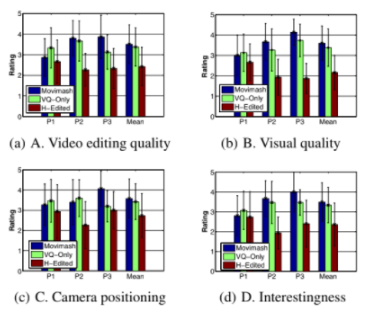
\includegraphics[width=0.5\textwidth]{img7.png}
    \caption{User responses for questions A, B, C, and D}
    \label{fig:figure7}
\end{figure}


\begin{figure}[h]
    \centering
    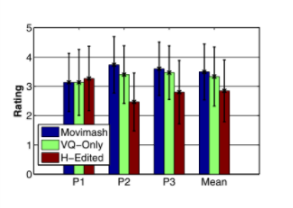
\includegraphics[width=0.5\textwidth]{img8.png}
    \caption{User response on overall quality of video}
    \label{fig:figure8}
\end{figure}


\section{EVALUATION}

The main goal of the experiments is to show that the proposed
framework produces a mashup with better view quality and diversity than earlier works. In addition, we also compare our result with
human-edited versions of mashups. The dataset consists of video
recordings of four performances. For each performance, we create three mashups: (1) using proposed framework (MoViMash) (2)
based on ranking average of shakiness, diversity, and video quality only (VQ-Only) (3) by human editor with editing experience (H-Edited). Users are asked to rate the quality of all three versions of mashup.

\subsection{Dataset}
The main application of the proposed framework is to combine
the videos recorded by mobile phone users. Therefore, we went to
three public performances and handed over smart phones to the audiences for recording. The audience were given a scenario where
they were recording the video for sharing with their friends who
were not present at the performance. All the performances happened during the night time. The video clips are converted to a
common resolution and synchronized before generating the mashups.
In this work, we synchronized the videos manually as our main focus is on video selection. The issue of automatic synchronization is
being researched separately \cite{14}. The details of the performances
and video recordings are given in the Table 2. Figure 6 shows selected frames for each performance.

\subsection{User Study}
In the user study, we ask the users to watch the mashups created
by the three methods and rate them accordingly. A total of seventeen users participated in the study, with age range from 20 to 30.
The users were mainly graduate students, males and females. The
three methods used to create the mashups were not disclosed to the
users. Further, the order of the videos produced by the different
methods was randomized for different performances to reduce the
bias the users may have due to particular presentation order.

The user study was conducted online with relevant instructions
explained beforehand. It is told to the users that "the main purpose
of this user study is to evaluate quality of video editing". Users
were asked to rate three distinct performance (P1, P2 and P3). The
three mashups (generated by MoViMash, VQ-Only and H-Edited)
are juxtaposed on a website with questions below them. The users were allowed to replay the videos while answering the questions.
The users rate the videos with a rating ranged between 1 to 5, where
1 represent worst and 5 being the best. The list of questions asked
are given in Table 3.


\subsection{Result Analysis}

The average responses of the users, along with their standard
deviations, are plotted in Figure \ref{fig:figure7} and Figure 8. We observed responses of the users for Questions A,B,C,D to be similar and with
slight variation for Question E.

\subsubsection{Analysis of Questions A, B, C, and D}
We observed that majority of users responded homogeneously
for all four of them. The responses indicated that the ratings were
based on some distinct characteristics of the video. Based on additional comments provided by the users, we infer that most of user
ratings were based on the quality of the selected video and coverage
of stage areas.

For P2 and P3, the users preferred the MoViMash created mashup.
For both the performances, user's found the shot transitions to be
smooth and pleasing. We relate this response of the user's to our
class-based learning for predicting the shot transitions. The users
also remarked that MoViMash produced videos had less occlusions
in comparison with VQ-Only based mashup.

While users liked MoViMash created mashups of P2 and P3,
they preferred VQ-Only mashup for P1. By analyzing the recordings and user comments, we found that P1 differs from P2 and P3 in
a common aspect. While P2 and P3 had a large number of similar
quality videos to select from at each time instant, the videos recordings of P1 were skewed with respect to quality. There were 2 to 3
videos which were stable and had very high video quality, whereas
all other videos were relatively bad in quality. Since MoViMash
attempts to maximize diversity along with video quality through
class-based shot selection, sometimes poor quality videos are selected.

On the other hand, P2 and P3 had many similar quality videos
to choose from, which allowed MoViMash to select videos of different classes with smooth transitions. Therefore, in the scenarios
where the quality of videos is skewed with only few good quality
videos, our MoViMash should be tuned to give more priority to
the quality rather than smooth transitions. The further tuning can
be done by selecting video from multiple future classes. However,
with proliferation of mobile camera, we envision that in future the
number of video recording will increase. An increased number of
recordings will ensure that there are sufficient number of reasonably good quality videos to ensure diversity of shots and smooth
transitions.

\begin{table}
	\caption{User study questions}
	\begin{tabular}{L{1cm}|L{7cm}} \hline
		\texttt A&Quality of video editing \\ \hline 
		\texttt B&Visual quality of video \\ \hline 
		\texttt C&Camera positioning in the video  \\ \hline
		\texttt D&Interestingness (does video editing makes an interesting overview of the performance?)\\ \hline
		\texttt E&Overall quality (how likely you will recommend the video to a friend?) \\ \hline
		
	\end{tabular}
\end{table}

The human-edited version received lowest ratings for all three
performances. After discussing with the human editor, we found
that most of video editing techniques they learn assume availability
of high quality videos. The video artifacts such as small camera shake, illumination variation etc. are generally negligible in these
high quality videos. Therefore, they are generally not comfortable
with the videos captured by mobile devices. Further, it would be
very difficult for a human editor to evaluate and precisely compare
quality of videos, particularly when the number of videos is large.
The performance of video editors can get even worse when they
have to make video selection in real-time. This finding makes a
strong case for automated mashup creation for live applications of
video sharing and broadcasting.

\subsubsection{Overall Video Quality}

User ratings for overall video quality are shown in the Figure 8.
We can see that on average, MoViMash outperforms other methods in overall video quality. Users generally liked the quality of
videos created by MoViMash for all three performances. Further,
the user ratings related to MoViMash had the least standard devi
ation among all three mashups. This result implies that the users
had highly correlated opinion about the superiority of MoViMash.
According to the comments users provided to justify their overall
video quality ratings, they liked following things about MoViMash:
complete coverage (from many angles), smooth shot transitions,
less occlusion, and balanced camera selection. Yet, there might
be instances where the semantics of the video govern the video
selection, e.g., celebrity appearance, funny behavior by crowd, interesting gestures and expressions by audiences, etc. It is hard for
the proposed automatic system to identify these instances; and a
human can be introduced in the selection to improve the mashup
quality in such scenarios.

It is important to note that although many users liked VQ-Only
created videos more than MoViMash, they did not specify any concrete aspect they liked about the video except selection of less
shaky videos. Thus, for the given dataset, even though VQ-Only
method is also able to produce videos with reasonable good quality,
it will fail in many real scenarios as it does not have any provision
for view quality and smooth shot transitions.

\subsection{Discussion}

The MoViMash framework takes automatic mashup creation methods closer to the human editors. It, however, adds to the processing
cost. The enhanced diversity model requires more memory for storing the history and more number of comparisons. Similarly, occlusion and tilt also require data processing that would have quadratic
complexity in terms of the number of pixels in the image. Therefore, individual components of the framework could be enabled or
disabled depending on the quality of the candidate videos. For example, if the videos are taken from the stand-mounted cameras,
shakiness calculation can be omitted. Furthermore, to make the
system scalable, we can process downscaled images as the video
resolution is not critical for the current system components.

\section{CONCLUSIONS \& FUTURE WORK}
In this paper, we have proposed and validated an online video
mashup creation framework, MoViMash, for videos recorded by
mobile devices. Based on the experiments and user study, we make
following conclusions:

\begin{itemize}
    \item MoViMash creates better quality mashups in comparison to
human editor, and other methods that are mainly based on
video quality.
\item Proposed learning framework is able to imitate professional
editor's experience to have smooth shot transitions in the final mashup. The proposed framework is most effective when there are a number of similar visual quality videos to chose from.
\item The proposed framework is able to filter occluded and tilted
views providing better viewing experience to the users.
\item Human editors are not comfortable in editing videos that are
recorded by mobile devices, particularly when there are large
number of videos with varying quality.
\item Proposed diversity model is able to incorporate both temporal and spatial aspects of the selection history.
\end{itemize}

In the future, we want to extensively evaluate individual components of the system with respect to end-to-end system delay and
output mashup quality. As current mobiles are capable of recording full HD video, we want to insert artificial zoom and pan in the
mashup using zoomable video techniques \cite{11}. Further, a human
director can only compare a limited number of videos at a time.
A powerful computer, however, can process and compare a large
number of videos simultaneously. Therefore, in the future we want
to study the impact of the number of videos on the quality of the
final mashup.

\section*{Acknowledgement}
This research is conducted under the NExT Search Center, supported by the Singapore National Research Foundation and the Interactive Digital Media R\&D Program Office of Media Development Authority under research grant WBS:R-252-300-001-490.




\bibliographystyle{ieeetr}
\bibliography{sig-alternate}


\end{document}



\grid
